\begin{frame}[t]
\centerline{
    \onslide<2->{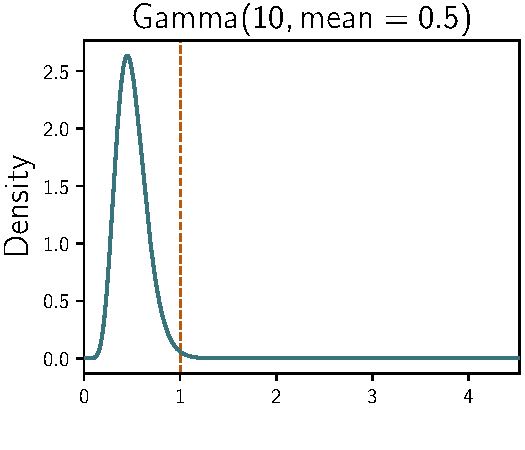
\includegraphics[width=0.34\linewidth]{../../simulations/validation/plots/relative-root-prior-10-005-gamma.pdf}}
    \hspace{-2.5mm}
    \onslide<2->{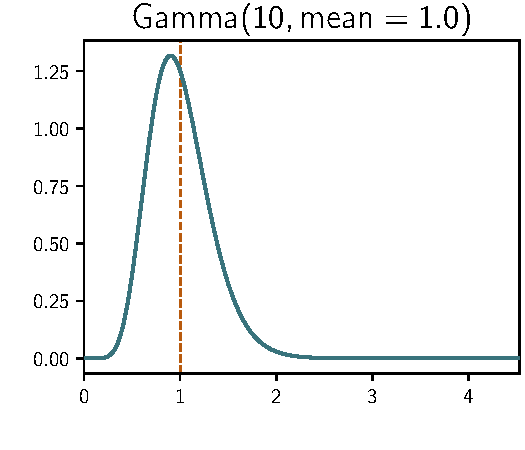
\includegraphics[width=0.34\linewidth]{../../simulations/validation/plots/relative-root-prior-10-010-gamma.pdf}}
    \hspace{-2.5mm}
    \onslide<2->{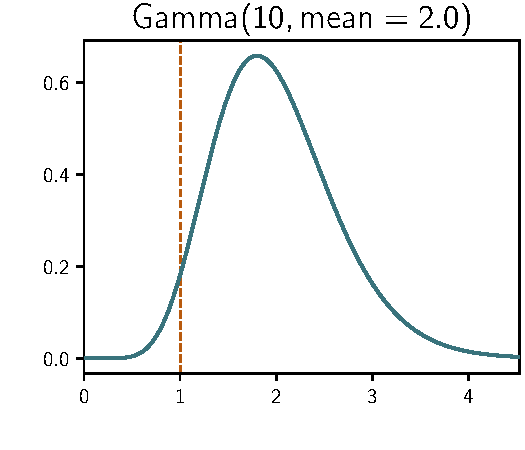
\includegraphics[width=0.34\linewidth]{../../simulations/validation/plots/relative-root-prior-10-020-gamma.pdf}}
}
\vspace{-4mm}
\centerline{
    \onslide<2->{Relative size of ancestral population}
}

\onslide<1->{
\begin{center}
    \LARGE
    \href{https://github.com/phyletica/ecoevolity}{
        \textbf{\textcolor{pgreen}{E}\textcolor{pteal}{co\textcolor{pauburn}{evo}lity}}}:
    \textcolor{pgreen}{\bf E}stimating \textcolor{pauburn}{\bf evo}lutionary \textcolor{pteal}{\bf coevality}
\end{center}
}

\onslide<1->{
\begin{itemize}
    \item Simulate datasets with 500k characters
    \item Use Bayesian model averaging with full
        likelihood\footnote[1]{\tiny\shortfullcite{Oaks2018ecoevolity}}$^,$\footnote[2]{\tiny\shortfullcite{Bryant2012}}
    \item No model misspecification
    \item $\textrm{\sffamily Time of change} \sim \textrm{\sffamily
            Exponential(\textrm{\sffamily mean} = 0.01)}$
\end{itemize}
}

\end{frame}

